\documentclass[10pt,a4paper]{article}
\usepackage{fullpage}
\usepackage{graphicx}
\usepackage{fancyhdr}
\setlength{\headheight}{13pt}
\pagestyle{fancy}

% default sans-serif
\renewcommand{\familydefault}{\sfdefault}

% no lines for headers and footers
\renewcommand{\headrulewidth}{0pt}
\renewcommand{\footrulewidth}{0pt}

% header
\fancyhf{}
\lhead{GWD-R}
\rhead{\today}

% footer
\lfoot{occi-wg@ogf.org}
\rfoot{\thepage}

% paragraphs need some space...
\setlength{\parindent}{0pt}
\setlength{\parskip}{1ex plus 0.5ex minus 0.2ex}

% some space between header and text...
\headsep 13pt

\setcounter{secnumdepth}{4}

\begin{document}

% header on first page is different
\thispagestyle{empty}

GWD-R \hfill  Thijs Metsch, Platform Computing\\
OCCI-WG \hfill  Andy Edmonds, Intel\\
\rightline {October 14, 2010}\\
\rightline {Updated: \today}

\vspace*{0.5in}

\begin{Large}
\textbf{Open Cloud Computing Interface - Core and Models}
\end{Large}

\vspace*{0.5in}

\underline{Status of this Document}

This document provides information to the community regarding the specification of the Open Cloud Computing Interface. Distribution is unlimited.

\underline{Obsoletes}

This document obsoletes GFD-xxx [REFERENCE].

\underline{Copyright Notice}

Copyright \copyright Open Grid Forum (2009-2010). All Rights Reserved.

\underline{Trademarks}

OCCI is a trademark of the Open Grid Forum.

\underline{Abstract}

This document, part of a document series, produced by the OCCI working group within the Open Grid Forum (OGF), provides a high-level definition of a Protocol and API. The document is based upon previously gathered requirements and focuses on the scope of important capabilities required to support modern service offerings. 

\newpage
\tableofcontents
\newpage

\section{Introduction}
The Open Cloud Computing Interface (OCCI) is a RESTful Protocol (and API) \marginpar{Probably no need for the brackets} for all kinds of Management tasks. OCCI was originally initiated to create a remote management API for IaaS model based Services, allowing for the development of interoperable tools for common tasks including deployment, autonomic scaling and monitoring. It now can be used to severe other models as well. To be modular and extensible the current specification itself is currently split into three complimentary documents:

\begin{itemize}
\item Core - this defines the OCCI model
\item HTTP Rendering - this defines how to manipulate the core model using the OCCI RESTful API. The document defines how the OCCI model can be communicated and thus serialized using HTTP.
\item Infrastructure - this defines the infrastructure domain resource types, the required attributes for each and the actions that can be taken on each.
\end{itemize}

\section{Notational Conventions}
All these parts and the information within are mandatory for implementors (unless otherwise specified). The key words "MUST", "MUST NOT", "REQUIRED", "SHALL", "SHALL NOT", "SHOULD", "SHOULD NOT", "RECOMMENDED", "MAY", and "OPTIONAL" in this document are to be interpreted as described in RFC 2119. 

\section{OCCI model}
OCCI is a boundary protocol/API \marginpar{Better as protocol and API} that acts as a service front-end to a provider’s internal management framework. Diagram \ref{fig:placement} shows OCCI's place in a provider’s architecture:

\begin{figure}[!hp]
	\centering
	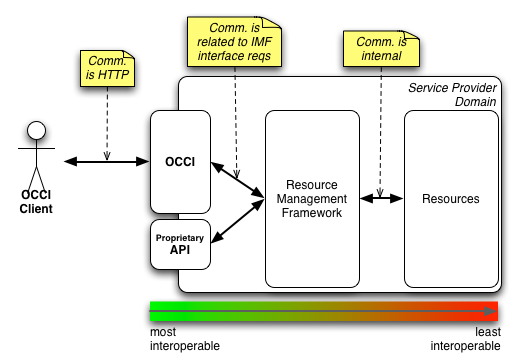
\includegraphics[scale=0.5]{figs/occi-intro.png}
	\caption{OCCI Overview}
	\label{fig:placement}
\end{figure}

The core of the OCCI model is simple. The central resource type is Resource and contains a number of common attributes that domain-specific Resource types inherit. These Resource types are complemented by two additional types, Link and Action. Accompanying these, Kind and Category provide the fabric for a safe extension model towards domain-specific usage. For compliance with OCCI Core, all types MUST be implemented. The UML class diagram \ref{fig:occi_core} gives an overview of the model.

\clearpage
\begin{figure}[!h]
	\centering
	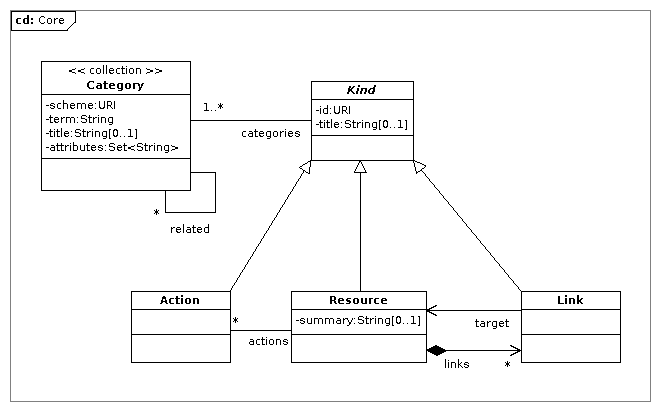
\includegraphics[scale=0.5]{figs/core_model.png}
	\caption{OCCI Overview}
	\label{fig:occi_core}
\end{figure}

The following sections of the specification define the foundations of the OCCI model, including common resource types, linkages and attributes.

\subsection{The base types}
The following sections describe the base types of the OCCI core model. The base types are Kind, Category, Resource, Link and Action. All base types MUST be implemented.

\subsubsection{Kind}
The Kind type is an abstract base type and common to all resources in the OCCI context. It MUST be implemented. Kind enforces for all subtypes a required id attribute and an (optional) title attribute. More importantly Kind introduces one or more type mix-ins through the type Category (see section \ref{sec:type_system}). The following table defines the attributes the Kind type MUST implement to be compliant:

\begin{tabular}{l|l|l|l|p{2.7in}}
Attribute & Type & Multiplicity & Client Access & Description \\
\hline
id & URI & 1 & read-many & Denotes a unique (within the service provider's name-space) identifier of a Kind subtype instance. \\
title & String & 0..1 & read-many/write-many & Denotes the display name of an instance. \\
categories & Category & 1..* & read-many & Comprises the Category types associated to this instance. Consumers can expect the attributes and actions of the associated Category types to be exposed by the instance. \\ 
\end{tabular}
\marginpar{should categories not be read-many/write-many?} 

\subsubsection{Category}
The Category type represent the classification mechanism used by OCCI. It MUST be implemented. From a system point of view a Category is used for two different classification purposes. See also section \ref{sec:type_system} ``Type System'' and section \ref{sec:collection} ``Collections''.

\begin{description}
\item[Taxonomy] A Category is used to assign static type information to each
resource type inheriting Kind or a descendant of Kind. This use of Category types
denotes the OCCI "static type system". A unique Category MUST be assigned to
every descendant of Kind. See the section \ref{sec:hierarchy} "Hierarchy".
\item[Folksonomy] A Category can be used to assign tags to resource instances
via a mix-in like model. A Category mix-in MUST NOT be related to an OCCI base
type (or any descendant of Kind) and MUST NOT be the unique identifier thereof.
Example use cases are collections, location information and templates for
virtual machine provisioning.
\end{description}

The following table defines the attributes the Category type MUST implement to be compliant:

\begin{tabular}{l|l|l|l|p{2.7in}}
Attribute & Type & Multiplicity & Client Access & Description \\
\hline
term & String & 1 & read-many & The category to which the resource belongs. \\
scheme & URI & 1 & read-many & The categorization scheme. \\
title & String & 0..1 & read-many & Denotes the display name of an instance. \\
attributes & String & 0..* & read-many & Comprise the resource attributes defined by the Category. \\
related & Category & 0..* & read-many & Set of related Category types. \\
\end{tabular}

A Category is uniquely identified by concatenating the categorization scheme with the category term, e.g. \textit{http://example.com/category/scheme\#term}. This is done to enable discovery of Category definitions per HTTP. All renderings MUST make use and understand concatenated unique identifiers of Category types.

\paragraph{Hierarchy}
\label{sec:hierarchy}
To be a part of the "static type system" a Category MUST be related, either directly or indirectly, to a base type Category. Extension of the OCCI base types through subtyping thus implies a hierarchy of related Category types.

In an example where "Custom-Compute-Resource" is a subtype of "Compute-Resource", which in turn is a subtype of the Resource base type, three related Category types would be involved. The following table illustrates the exemplified hierarchy of Category types relating the custom Category to a base type Category.

Example:

\begin{tabular}{p{0.6in}|p{3.1in}|p{2in}}
Kind & Category & Related Category \\
\hline
Custom-Compute-Resource & \textit{http://example.com/occi/custom\#compute} & \textit{http://schemas.ogf.org/occi/infrastructure\#compute} \\
Compute-Resource & \textit{http://schemas.ogf.org/occi/infrastructure\#compute} & \textit{http://schemas.ogf.org/occi/core\#resource} \\
Resource & \textit{http://schemas.ogf.org/occi/core\#resource} & none \\
\end{tabular}

\subsubsection{Resource}
The Resource type describes a concrete resource that can be inspected and manipulated. It represents a general object in the OCCI core model and MUST be implemented. Resource enforces the inheritance of a set of common attributes into subtypes (such as a unique identifier and an optional descriptive summary). Moreover, it introduces relationships to other Kind instances, denoted by Links. It also introduces operations that can be invoked on this instance, denoted by Actions.

The Resource type is assigned the \textit{http://schemas.ogf.org/occi/core\#resource} Category.

\begin{itemize}
  \item A Resource instance MUST at least expose this or a related Category together with any associated attributes.
  \item A Resource instance MUST advertise those of its Actions, if any, which are currently applicable.
  \item A Resource instance MUST implement the attributes in the following table:
\end{itemize}

\begin{tabular}{l|l|l|l|p{2.7in}}
Attribute & Type & Multiplicity & Client Access & Description \\
\hline
summary & String & 0..1 & read-many/write-many & Holds a summarizing description of the Resource instance.\\
links & Link & 0..* & read-many/write-many & Comprises a set of Link compositions. Being a composite relation the removal of a Link from the set MUST also remove the Link instance.\\
actions & Action & 0..* & read-many & Set of Actions associated with the Resource.\\
\end{tabular}

The OCCI Extension documents define sets of specific subtypes of Resources, Links and Actions. They inherit Resource and is each assigned an unique Category.

\subsubsection{Link}
The Link type defines a base association between two Resources. It MUST be implemented. Link indicates that one resource is connected to another.

The Link type is assigned the \textit{http://schemas.ogf.org/occi/core\#link Category}. A Link instance MUST at least expose this or a related Category together with any associated attributes. A Link instance MUST also implement the attributes in the following table:

\begin{tabular}{l|l|l|l|p{2.7in}}
Attribute & Type & Multiplicity & Client Access & Description \\
\hline
target & Resource & 1 & read-many/write-many & Denotes the resource this instance points to.\\
\end{tabular}
\marginpar{Open issue: should 'source' be here or in the http section. Semantic versus syntax issue.} 

The Link base type MUST NOT refer to an external resource. A provider MAY however create a subtype of Link with different semantics that e.g. have a target attribute containing an URI and thus the ability of linking with external resources.

\subsubsection{Action}
The Action type defines an invocable operation on an associated Resource. It MUST be implemented. In general, Actions modify state (e.g. by performing a complex operation such as rebooting a virtual machine).

The Action type is assigned the \textit{http://schemas.ogf.org/occi/core\#action} Category. An Action instance MUST at least expose this or a related Category together with any associated attributes.

\subsection{Mutability}
\marginpar{Does 'client access' need to be discussed here?} 
Attributes of a OCCI base type instance, a resource instance, are either client mutable or client immutable. If an attribute is noted to be mutable this MUST be interpreted that a client can create a resource instance that is parametrized by the attribute. Likewise, if an attribute is mutable, a client can update that resource instance's mutable attribute value and the server side MUST support this. If an attribute is marked as immutable, it indicates that the server side implementation MUST manage these exclusively. Immutable attributes MUST NOT be modifiable by clients under any circumstance.

\subsection{Type System}
\label{sec:type_system}
The Category type is the classification mechanism used by OCCI. This tells service providers what type of concrete OCCI Kind should be created. Each domain-specific section of the OCCI specification (e.g. infrastructure) defines its own concrete Resource, Action and optionally Link specializations. It should be noted that depending on a client's credentials, access to creating certain OCCI Kind instances MAY be restricted.

The type system is a flexible and extensible one allowing for the addition of "mix-in" Category types. Mix-in Category types are ones that add additional behavior to OCCI Kinds and are Category types not defined by the OCCI specifications. The mix-in Category types can be added to an OCCI Kind both at Kind creation-time and run-time. The Kinds to which a particular mix-in Category type can be applied, is defined by the provider implementation. At which time, creation- or run-time, these mix-in types can be applied is also defined by the provider implementation. Discovery of mix-in types can be achieved by querying the OCCI Query interface. Mix-in Category types are those that are NOT related to an OCCI base type Category and MUST be implemented as such. When a client attempts to add a mix-in at a stage not supported by the provider, the provider MUST notify the client that it has issued a bad request.

\subsubsection{Creating Instances}
A client MUST supply the concrete Kind type as a Category. All OCCI implementations MUST understand these requests containing concrete Kind types, i.e. Resource, Link, Action or a subtype thereof.

\subsection{Collections}
\label{sec:collection}

One or more Kind sub-type instances assigned to the same Category automatically
form a collection. Each Category in the system identifies a collection
consisting of all different Kind instances associated with the Category.

A Kind sub-type instance is always a member of the Kind's identifying Category
collection since a Kind instance MUST be assigned the Kind sub-type Category.
Since a tag Category can be assigned to any Kind instance a collection can
contain instances of different Kind sub-types.

For example an instance of the Resource type will be assigned the
\textit{http://scheme.ogf.org/occi/core\#resource} Category and thus part of the
Resource Category collection.


\subsection{Extensibility}
The OCCI Core model has a flexible yet fairly simple extension mechanism through the use of sub-typing and Category types. 

\subsubsection{Sub-types and Category Types}
The OCCI Core model has a flexible yet fairly simple extension mechanism through the use of sub-typing and Category types.
A provider MAY extend the OCCI core model by creating a subtype of either an OCCI Core base type or a provider defined subtype.

A provider MUST assign a new unique Category to each new subtype defined. The new Category MUST be, either directly or indirectly, related to one of the Core base types, i.e. Resource, Link or Action. If a provider extends a subtype the new Category SHOULD be related to the subtype extended, provided the previous rule holds true.

Providers MAY also define new Category types for tagging and templating purposes. Such a Category MUST NOT be the unique identifier of a resource type, i.e. must not be part of the "static type system".

The scheme of provider-defined Category types MUST reside in a unique namespace different from those in the OCCI specification. Any attributes defined by a new Category MUST NOT have a name starting with occi. The occi namespace prefix is reserved for extensions which are standardized. A provider SHOULD use an attribute namespace comprising the reverse domain name as prefix to every attribute name.

A provider-defined Category identifying a custom subtype of Resource could be exemplified as follows. The term and scheme is defined by the provider. The related set MUST include a, direct or indirect (through a hierarchy), reference to the Resource base type category.

\begin{itemize}
\item term = custom\_resource.
\item scheme = \textit{http://example.com/occi/resource\#}
\item related = \textit{http://schemas.ogf.org/occi/core\#resource}
\end{itemize}

\subsubsection{Extension of the base types}
A provider MAY define subtypes of the Core base types Resource, Link and Action for domain-specific purposes. A unique Category MUST be assigned to each new subtype. The assigned Category MUST be directly related to the Category of the base type extended.

\subsubsection{Extension of subtypes}
A provider MAY define subtypes of any existing subtype, either defined in OCCI or by someone else. A unique Category MUST be assigned to each new subtype. The assigned Category MUST be either directly or indirectly related to a base type Category. It is RECOMMENDED the Category is related to the Category of the subtype extended.

\subsection{Discovery}
An OCCI client MUST be able to discover all Category types a particular provider supports before interacting with the provider. Since the rendering of the Category types is depended of the protocol the rendering documents give more information on how information is send and can be parsed.

\section{Contributors}
Editors: Andy Edmonds, Thijs Metsch \\
Contributors: Alexander Papaspyrou, Ralf Nyrén, Sam Johnston

\textbf{TBD: Bunch op people missing here - create table\ldots}

\section{Glossary}

\begin{tabular}{l|l}
Term & Description \\
\hline
OCCI & Open Cloud Computing Interface \\
\end{tabular}

\section{Intellectual Property Statement}

The OGF takes no position regarding the validity or scope of any intellectual property or other rights that might be claimed to pertain to the implementation or use of the technology described in this document or the extent to which any license under such rights might or might not be available; neither does it represent that it has made any effort to identify any such rights. Copies of claims of rights made available for publication and any assurances of licenses to be made available, or the result of an attempt made to obtain a general license or permission for the use of such proprietary rights by implementers or users of this specification can be obtained from the OGF Secretariat.

The OGF invites any interested party to bring to its attention any copyrights, patents or patent applications, or other proprietary rights which may cover technology that may be required to practice this recommendation. Please address the information to the OGF Executive Director.

\section{Disclaimer}

This document and the information contained herein is provided on an ''As Is'' basis and the OGF disclaims all warranties, express or implied, including but not limited to any warranty that the use of the information herein will not infringe any rights or any implied warranties of merchantability or fitness for a particular purpose.

\section{Full Copyright Notice}

Copyright \copyright Open Grid Forum (2009-2010). All Rights Reserved.

This document and translations of it may be copied and furnished to others, and derivative works that comment on or otherwise explain it or assist in its implementation may be prepared, copied, published and distributed, in whole or in part, without restriction of any kind, provided that the above copyright notice and this paragraph are included on all such copies and derivative works. However, this document itself may not be modified in any way, such as by removing the copyright notice or references to the OGF or other organizations, except as needed for the purpose of developing Grid Recommendations in which case the procedures for copyrights defined in the OGF Document process must be followed, or as required to translate it into languages other than English.

The limited permissions granted above are perpetual and will not be revoked by the OGF or its successors or assignees.

\section{References}

Note that only permanent documents should be cited as references. Other items, such as Web pages or working groups, should be cited inline (i.e., see the Open Grid Forum, http://www.ogf.org). References should conform to a standard such as used by IEEE/ACM, MLA, Chicago or similar. Include an author, year, title, publisher, place of publication. For online materials, also add a URL. It is acceptable to separate out ''normative references,'' as IETF documents typically do. Some sample citations: 

\end{document}
